\section{k-Nearest Neighbour classification on mixed datasets}
\label{sec:knnmulti}
With data from 10 individuals
\(D_{MULTI}=G1M1\cup G2M1\cup G3M1\cup G4M1\cup G5M1\cup G6M1\cup G7M1\cup G8M1\cup G10M1\cup G11M1\),
downsampled to 100 DPI and smoothed with \(\sigma=1.5\),
k-NN classification accuracy was measured using 10-fold cross validation (3 runs),
for \(k=1,2,3,5,7,11,30,40,80\).
The data was split into training and testing data in two different ways:

\begin{itemize}
	\item \textbf{MIX}: Data from all individuals in \(D_{MULTI}\)
	is contained in both training and testing sets.
	\item \textbf{LOO}: Leave one out - Individual \(GXM1\) is
	left out of the training data in each cross validation run with
	training set equal to \(D_{MULTI}\setminus GXM1\) and testing set equal to \(GXM1\).
\end{itemize}

The results can be seen in figure \ref{fig:knn-acc-multi}.

\begin{figure}[ht]
	\centering
	\begin{subfigure}[t]{0.9\textwidth}
		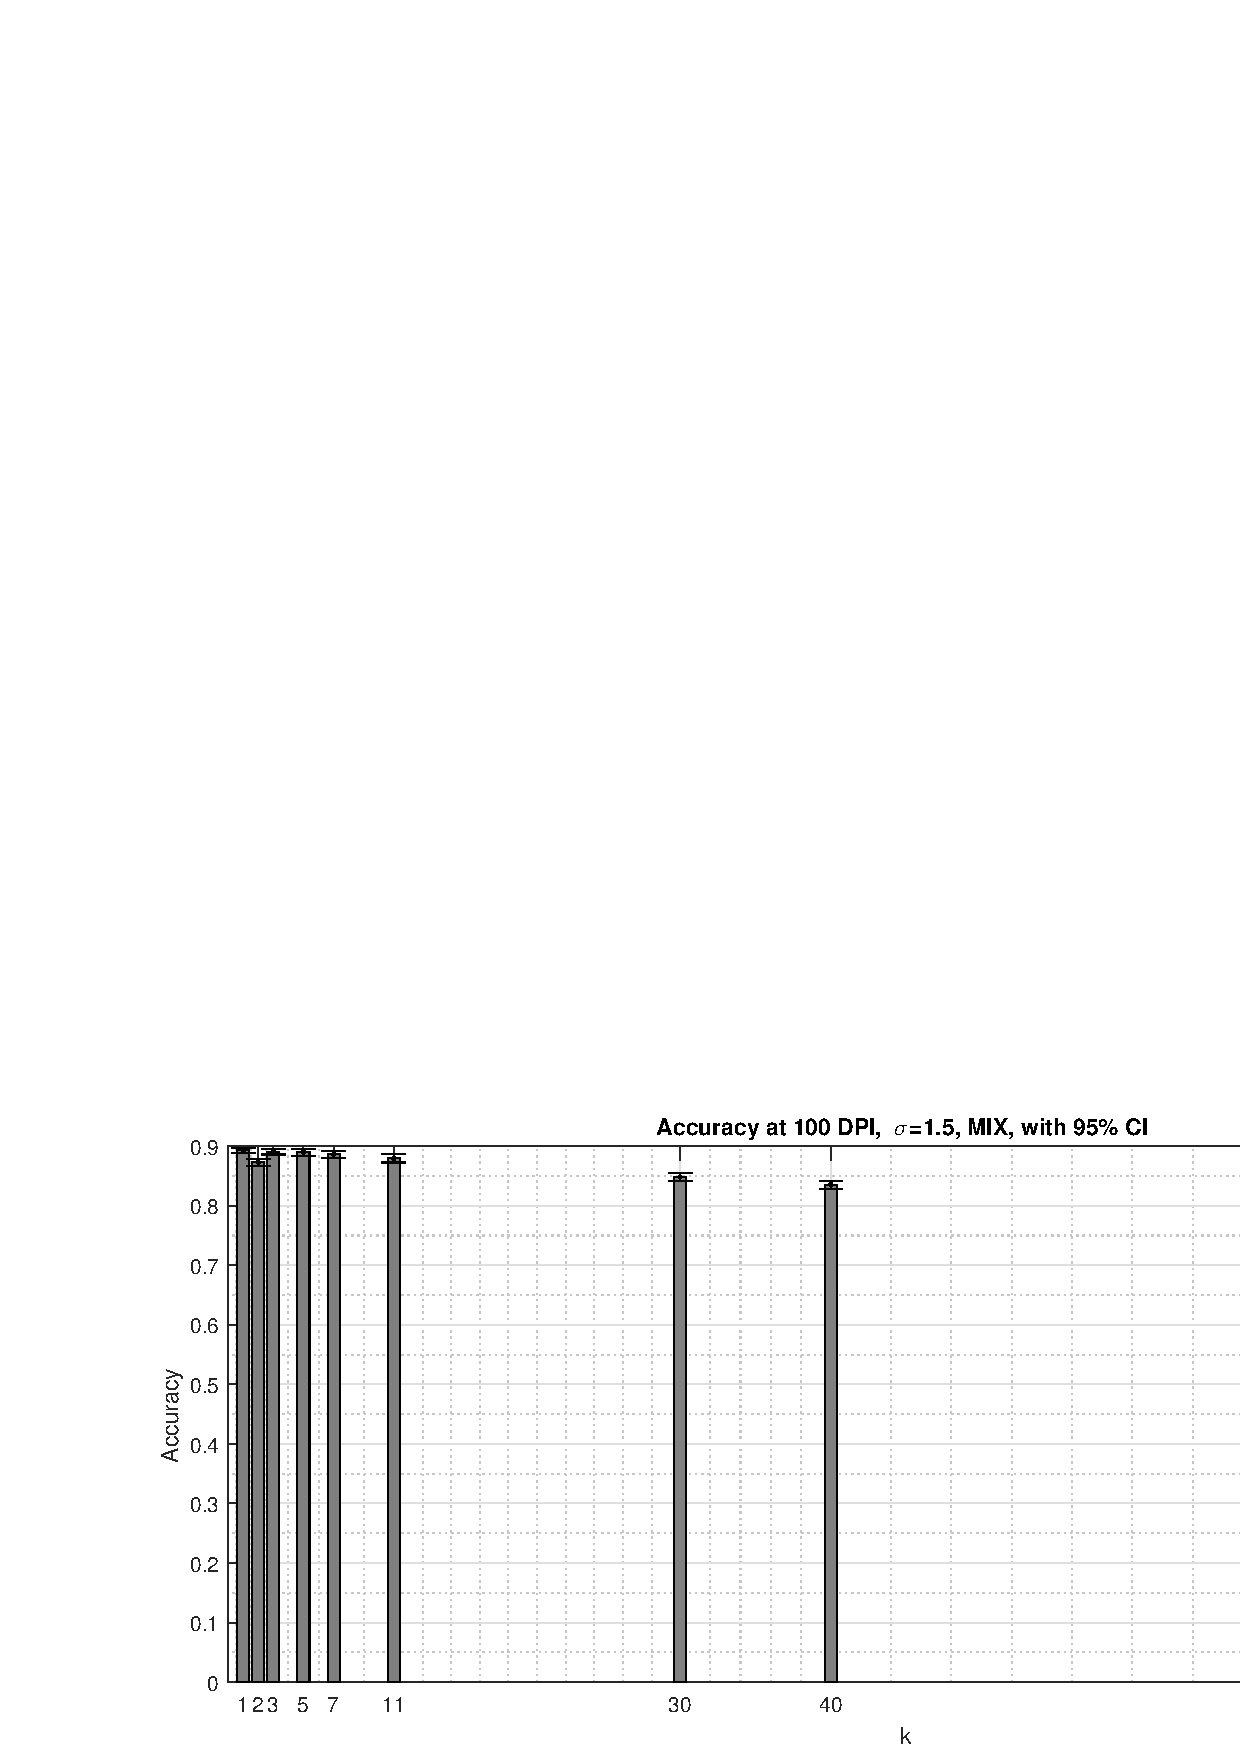
\includegraphics[width=\textwidth]{{{graphics/knn-acc-multiMIX-dpi100-sig1.5}}}
		\caption{\textbf{MIX}.}
	\end{subfigure}
	\begin{subfigure}[t]{0.9\textwidth}
		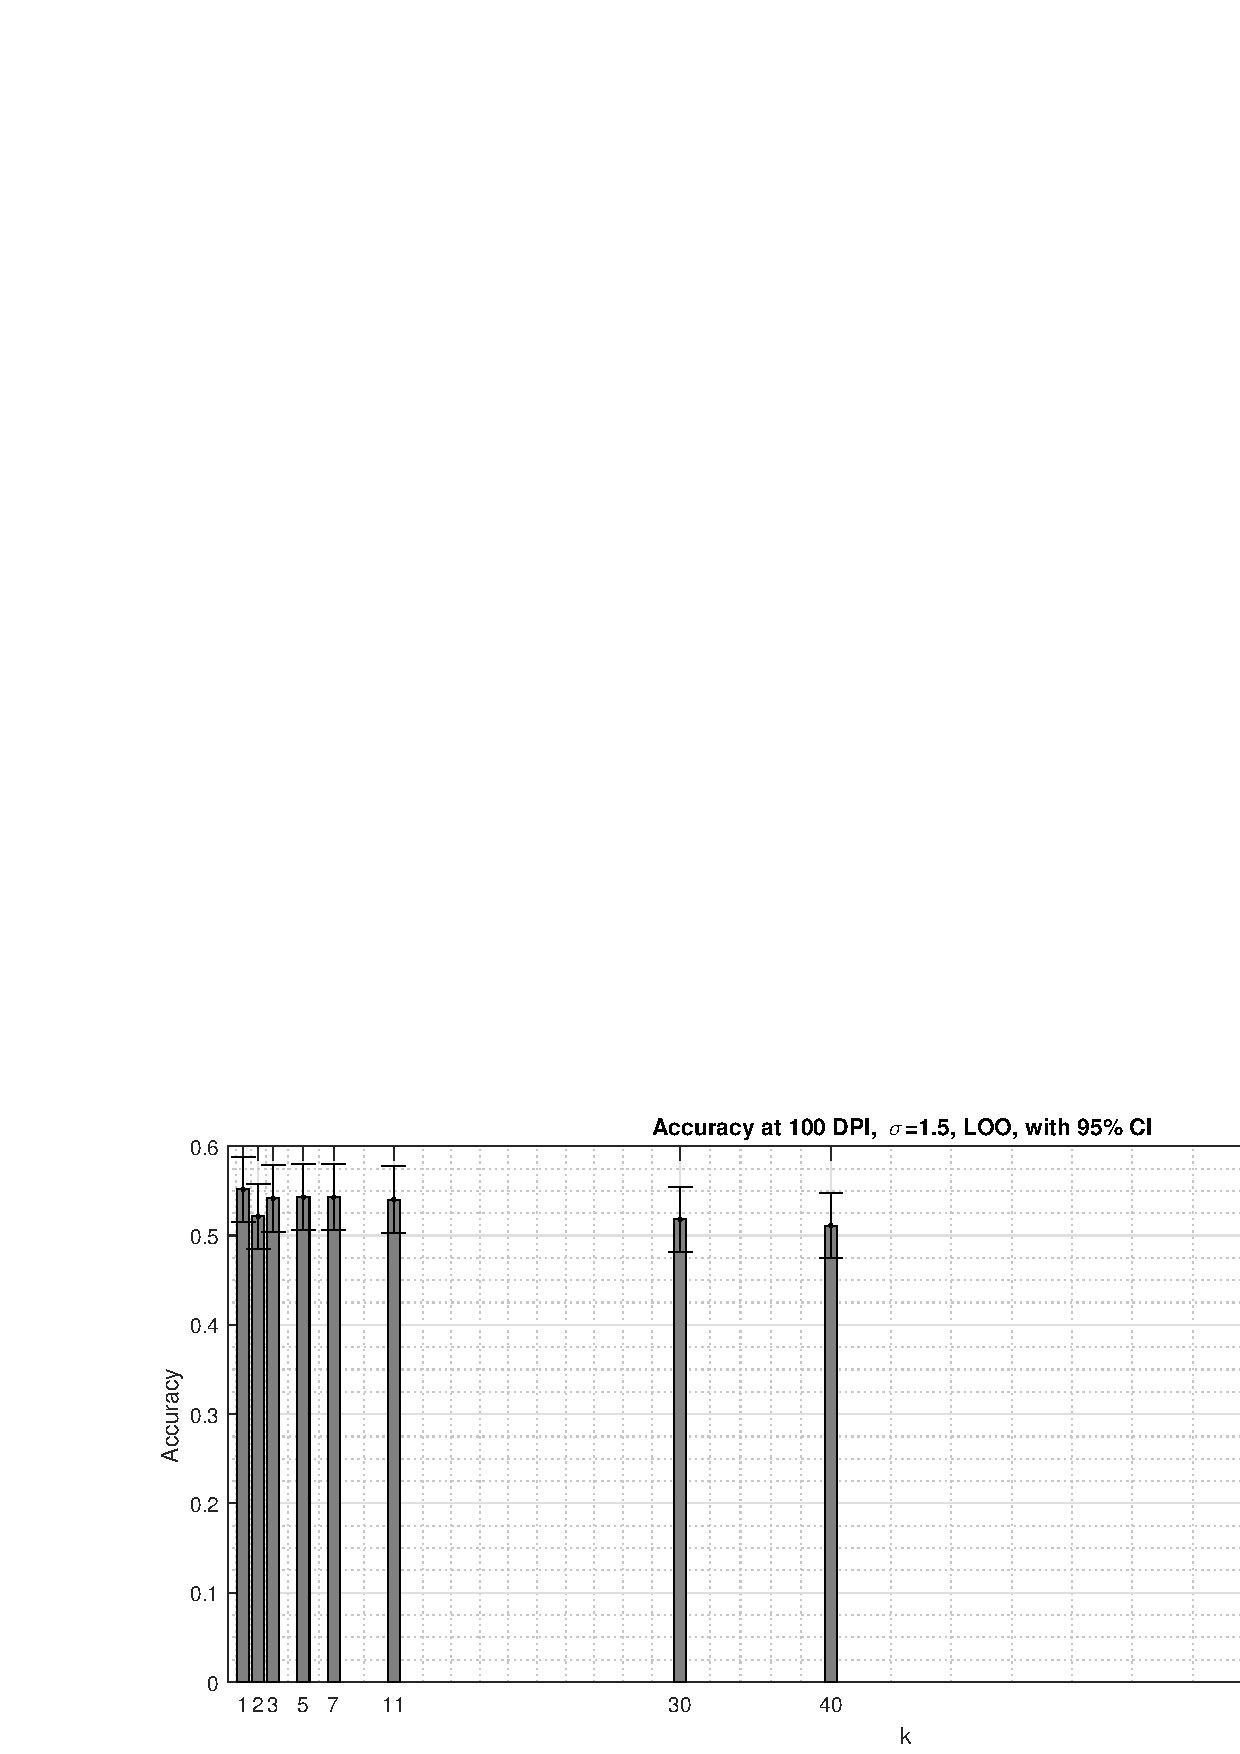
\includegraphics[width=\textwidth]{{{graphics/knn-acc-multiLOO-dpi100-sig1.5}}}	
		\caption{\textbf{LOO}.}
	\end{subfigure}
	\caption{
		k-NN classification accuracy vs. k for \(D_{MULTI}\).
		Based on 3 runs of 10-fold cross validation.
	}
	\label{fig:knn-acc-multi}
\end{figure}

Figure \ref{fig:confmatknn-multi} shows example confusion matrices for
\textbf{MIX} and \textbf{LOO} (\(D_{MULTI} \setminus G1M1\)).

\begin{figure}[ht]
	\centering
	\begin{subfigure}[t]{0.45\textwidth}
		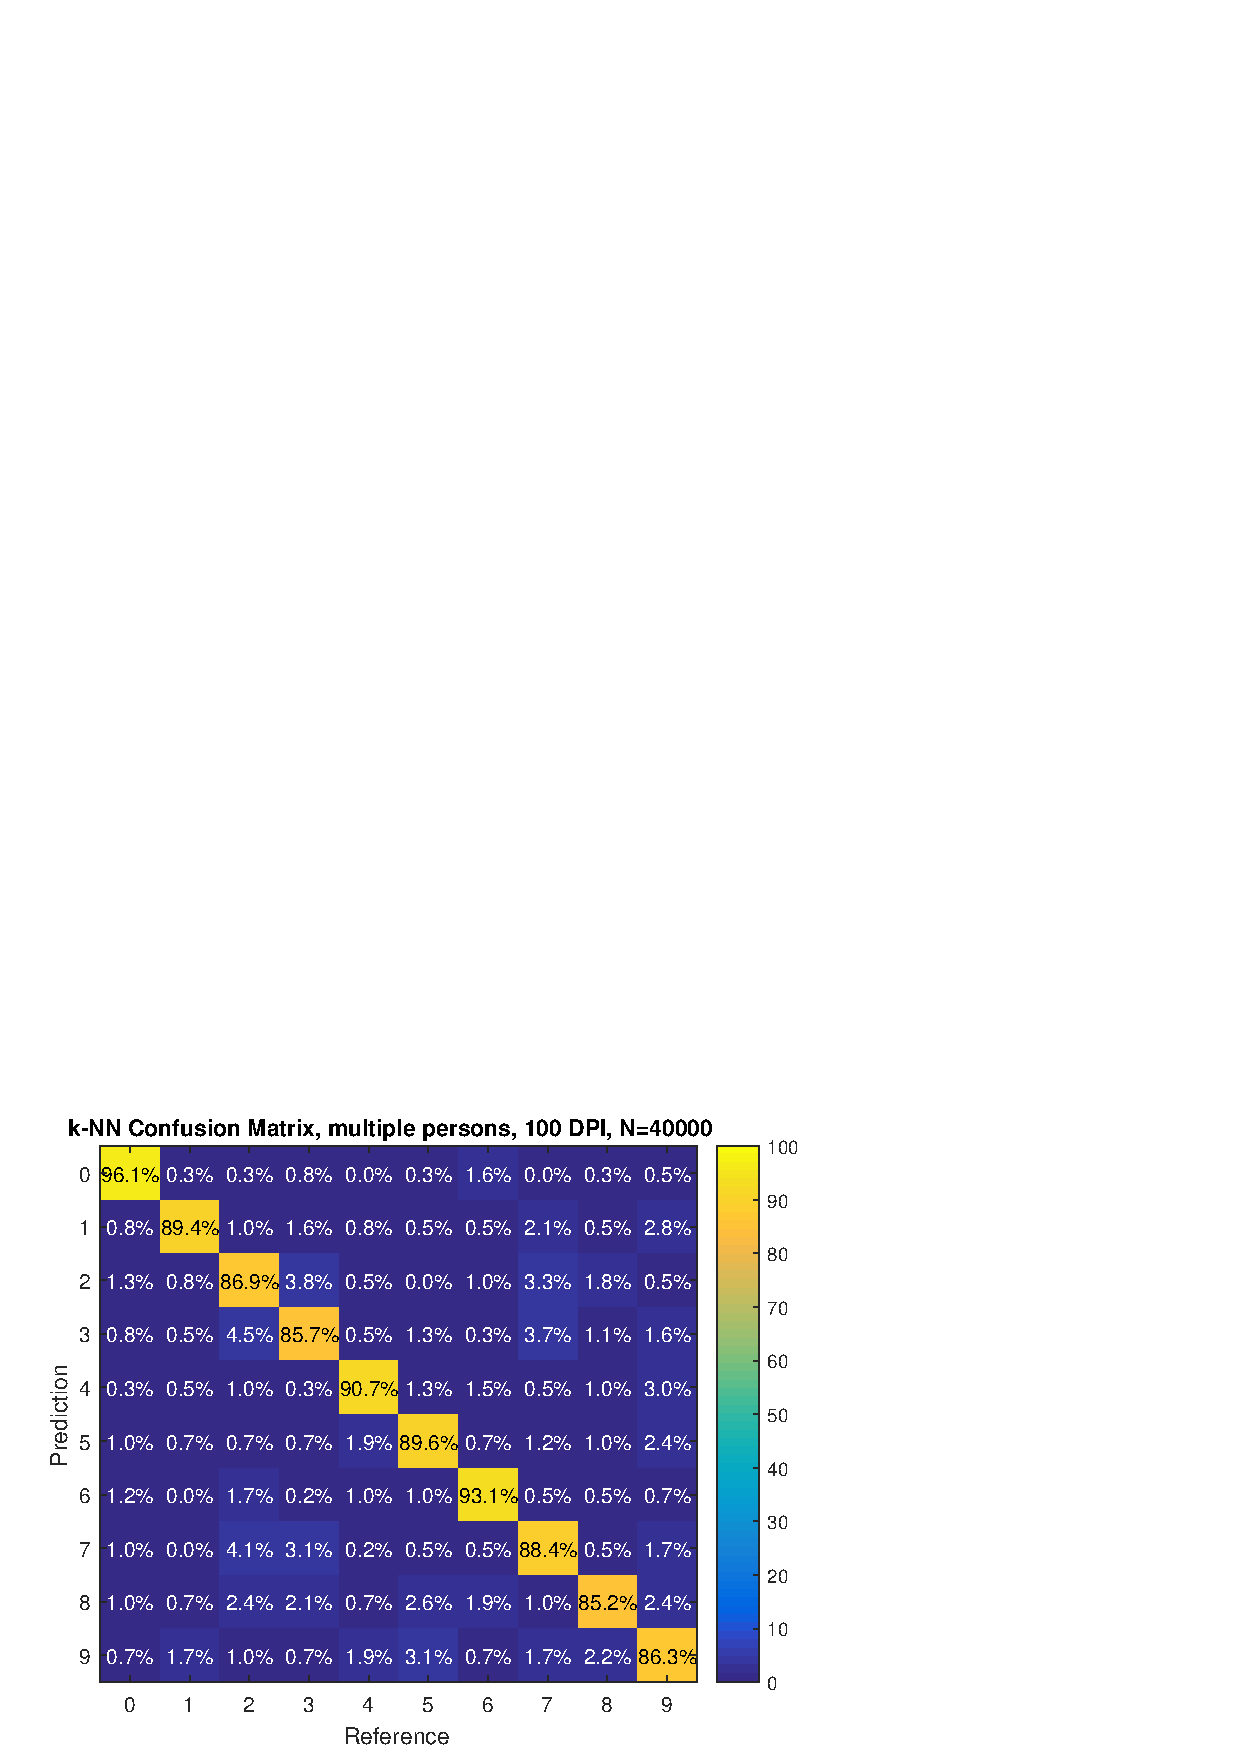
\includegraphics[width = \textwidth]{{{graphics/confmatkNN-multiAll-sig1.5-k1-n40000}}}
		\caption{\textbf{MIX}.}
	\end{subfigure}
	\begin{subfigure}[t]{0.45\textwidth}
		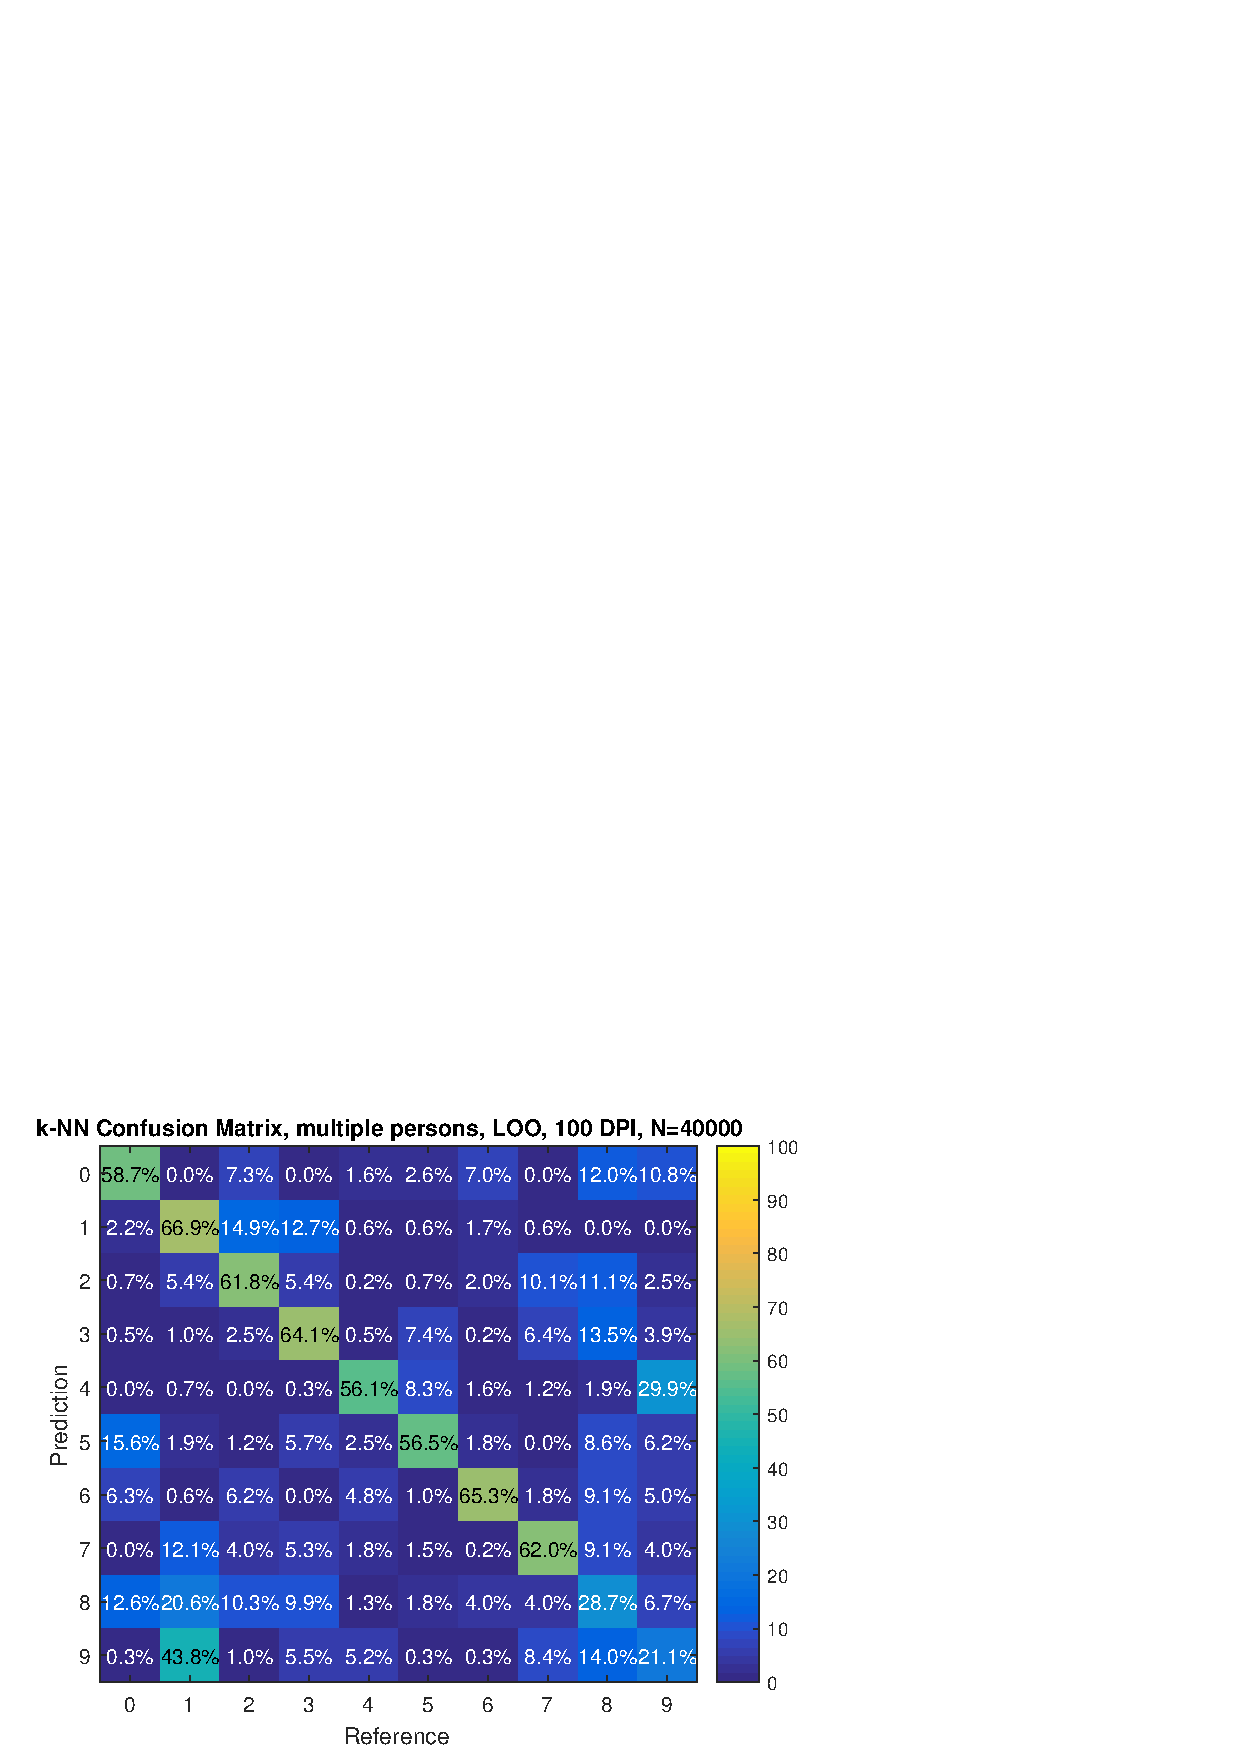
\includegraphics[width = \textwidth]{{{graphics/confmatkNN-multiLOO-sig1.5-k1-n40000}}}
		\caption{\textbf{LOO}. \(D_{MULTI} \setminus G1M1\) training set.}
		\label{fig:confmatknn-multiLOO}
	\end{subfigure}
	\caption{
		Example confusion matrices for k-NN with \(k=1\) and \(\sigma=1.5\) at 100 DPI for \(D_{MULTI}\).
	}
	\label{fig:confmatknn-multi}
\end{figure}

Figure \ref{fig:knn-acc-multi} shows that for the tested values of \(k\),
\(k=1\) yields highest accuracy as with the G2M2 dataset,
in both the \textbf{LOO} and the \textbf{MIX} configurations.
Figure \ref{fig:knn-acc-multi} also clearly shows that the \textbf{LOO} configuration
yields much lower accuracy than the \textbf{MIX} configuration.